\chapter{Installation of Unitex}
\label{chap-install}

Unitex is a multi-platform system that runs on Windows as well as on Linux or
MacOS. This chapter describes how to install and how to launch Unitex on any of
these systems. It also presents the procedures used to add new languages and to
uninstall Unitex.

\section{Licenses}

\index{LGPL}\index{License!LGPL}
Unitex is a free software. This means that the sources of the programs are
distributed with the software, and that anyone can modify and redistribute them.
The code of the Unitex programs is under the LGPL licence (\cite{LGPL}), except
for the TRE library for dealing with regular expressions from Ville Laurikari
(\cite{TRE}), which is under 2-clause BSD licence which is more
permissive than the LGPL. The LGPL Licence is more permissive than the GPL
licence, because it makes it possible to use LGPL code in nonfree software. 
From the point of view of the user, there is no difference,
because in both cases, the software can freely be used and distributed.

\bigskip
\noindent All the data that go with Unitex are distributed under the LGPLLR
license \index{LGPLLR} (\cite{LGPLLR}).

\bigskip
\noindent Full text versions of LGPL, 2-clause BSD and LGPLLR can be found in
the appendices of this manual.

\section{Java runtime environment}
Unitex consists of a graphical interface written in Java and external programs
written in \textit{C/C\kern-.05em\raisebox{.5ex}{++}\kern-.1em}. This mixture of
programming languages is responsible for a fast and portable application that
runs on different operating systems.

\bigskip
\noindent Before you can use the graphical interface, you first have to install the runtime
environment, usually called Java virtual machine \index{Java virtual machine} or
JRE\index{JRE} (Java Runtime Environment\index{Java Runtime Environment}).

\bigskip
\noindent For the graphical mode, Unitex needs Java version 1.6 (or newer). If you have an
older version of Java, Unitex will stop after you have chosen the working
language.

\bigskip
\noindent You can download the virtual machine for your operating system for free from the
Sun Microsystems web site (\cite{site-java}) at the following address:
\url{http://java.sun.com}.

\bigskip
\noindent If you are working under Linux or MacOS, or if you are using a Windows version
with personal user accounts, you have to ask your system administrator to install
Java.

\section{Installation on Windows}
\index{Installation!on Windows}
If Unitex is to be installed on a multi-user Windows machine, it is recommended
that the systems administrator performs the installation. If you are the only
user on your machine, you can perform the installation  yourself.

\bigskip
\noindent Decompress the file \index{File!\verb+unitex_2.0.zip+} \verb+unitex_2.0.zip+ (You
can download this file from the following address:
\url{http://www-igm.univ-mlv.fr/~unitex}) into a directory \verb+Unitex+ that
should preferably be created within the \verb+Program Files+ folder.

\bigskip
\noindent After decompressing the file, the \verb+Unitex+ directory contains several
subdirectories  one  of which is called \verb+App+. This directory contains a
file called \verb+Unitex.jar+. \index{File!\verb+Unitex.jar+} This file is the
Java executable that launches the graphical interface. You can double click on
this icon to start the program. To facilitate launching Unitex, you may want to
add a shortcut to this file on the desktop.

\section{Installation on Linux and Mac OS X}
\index{Installation!on Linux and Mac OS X}
In order to install Unitex on Linux, it is recommended to have system
administrator permissions. Uncompress the file \verb+Unitex2.1.zip+ in a
directory named \verb+Unitex+, by using the following command:

\bigskip \noindent \verb$unzip Unitex2.1.zip -d Unitex$

\bigskip
\noindent Within the directory \verb|Unitex/Src/C++/build|, start the compilation
of Unitex with the command:

\bigskip \verb+make install+

\bigskip
\noindent or with the following if you have a 64 bits computer:
 
\bigskip \verb+make install 64BITS=yes+

\bigskip
\noindent You can then create an alias in the following way:

\bigskip \verb$alias unitex='cd /..../Unitex/App/ ; java -jar Unitex.jar'$

\section{First use}
If you are working on Windows, the program will ask you to choose a
\index{Directory!personal working} personal working  directory, which you can
change later in "Info>Preferences...>Directories". To create a directory, click
on the icon showing a file (see
figure~\ref{fig-creation-personal-directory}).

\bigskip
\noindent If you are using Linux or MacOS, the program will automatically create a
\verb+/unitex+ directory in your \verb+$HOME+ directory. This directory allows
you to save your personal data. For each language that you will be using, the
program will copy the root directory of that language to your personal
directory, except the dictionaries. You can then modify your copy of the
files without risking to damage the system files.

\begin{figure}[h]
\begin{center}
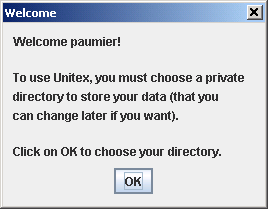
\includegraphics[width=6.3cm]{resources/img/fig1-1.png}
\caption{First use under Windows}
\end{center}
\end{figure}

\begin{figure}[h]
\begin{center}
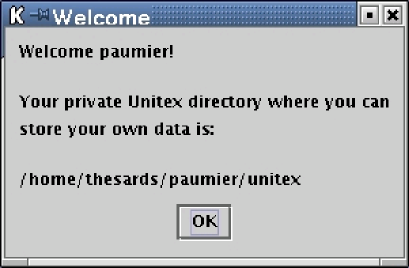
\includegraphics[width=7cm]{resources/img/fig1-2.png}
\caption{First use under Linux}
\end{center}
\end{figure}

\begin{figure}[h]
\begin{center}
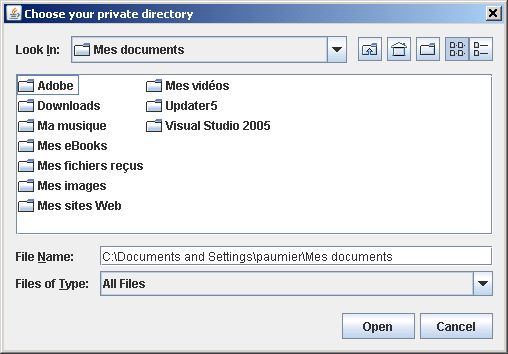
\includegraphics[width=13cm]{resources/img/fig1-3.png}
\caption{Creating the personal work
directory\label{fig-creation-personal-directory}}
\end{center}
\end{figure}


\section{Adding new languages}
\index{Adding languages}

\bigskip
\noindent There are two different ways to add languages. If you want to add 
a language that is to be accessible by all  users, you have to copy the 
corresponding directory to the \verb+Unitex+ system directory, for which 
you will need to have the access rights  (this might mean that you need to 
ask your system administrator to do it). On the other hand, if the language 
is only used by a single user, he can also copy the directory to his working 
directory. He can work with this language without this language being shown to other users.


\section{Uninstalling Unitex}
No matter which operating system you are working with, it is sufficient to delete 
the \verb+Unitex+ directory to completely delete all the program files. Under
Windows you may have to delete the shortcut to \verb+Unitex.jar+ \index{File!\verb+Unitex.jar+} 
if you have created one on your desktop. The same has to be done on Linux, if you have 
created an alias.
